\subsection{Using a Neural Network}
We end up using a very simple network (\Cref{table:simple-network}) to complete our task (Other, more complex networks were experimented on and the results are compiled in \Cref{Appendix:Networks}).
We call our network \it{ARAMNet}, since our motivations came from the game of ARAM.

\begin{table}[htbp]
    \centering
    \bgroup
    \def\arraystretch{1.5}
    \begin{tabular}{|c|c|c|c|}
        \hline
        Layer       & Kernel Shape & Output Shape & \# Params \\
        \hline
        LSTM        &              & (10, 152)    & 186.048k  \\
        \hline
        BatchNorm   & (10, 1)      & (10, 152)    & 20        \\
        \hline 
        Flatten     &              & (1, 1520)    &           \\ 
        \hline
        Linear      & (1520, 1520) & (1, 1520)    & 2.31192M  \\ 
        \hline
        Reshape     &              & (10, 152)    &           \\ 
        \hline
        Softmax     &              & (10, 152)    &           \\ 
        \hline
    \end{tabular}
    \egroup
    \caption{ARAMNet}
    \label{table:simple-network}
\end{table}

The most important part we had to design into our network was the ordering of the players.
It had to be the case that if we modified the ordering, the output would reflect the change as well.
(Unless, of course, our particular instance was order-invariant)
This naturally led us to the idea of treating the $10$ players as temporal sequence of data instead of just a matrix of pool encodings.
More precisely (for those familiar with RNN-related notation), our input data is a sequence of $10$ players: $(P^{<1>}, \ldots, P^{<10>})$, which we feed into an initial layer of LSTM cells.
The network then outputs a $10$-by-$152$ matrix $M$ where $M_{ij} := \Pr(P_i \text{ selects } j)$ (i.e. The rows are precisely the discrete probability distribution for player $P_i$), performing exactly what our simulator was doing.

Although we said we would replace the simulator, we use it here one last time to generate $6000$ samples for our network to train on.
Our goal here is to minimize the Hellinger distance between the network output and simulator output, and we achieve a final training loss of $0.025$ and validation loss of $0.035$.
We train using AdamW with all the recommended settings, except for an increase in the weight decay to $0.25$, and a batch size of 16.
The learning rate was adjusted using \it{ReduceLROnPlateau}\footnote{See \url{https://pytorch.org/docs/stable/_modules/torch/optim/lr_scheduler.html\#ReduceLROnPlateau}}, a built-in Pytorch learning rate scheduler, with a patience of $4$ and a threshold of $0.01$.
The adjusting learning rate produces the bumps we see in \Cref{Figure:ARAMNet-Learning-Curve}.

\begin{figure}[htbp]
    \centering
    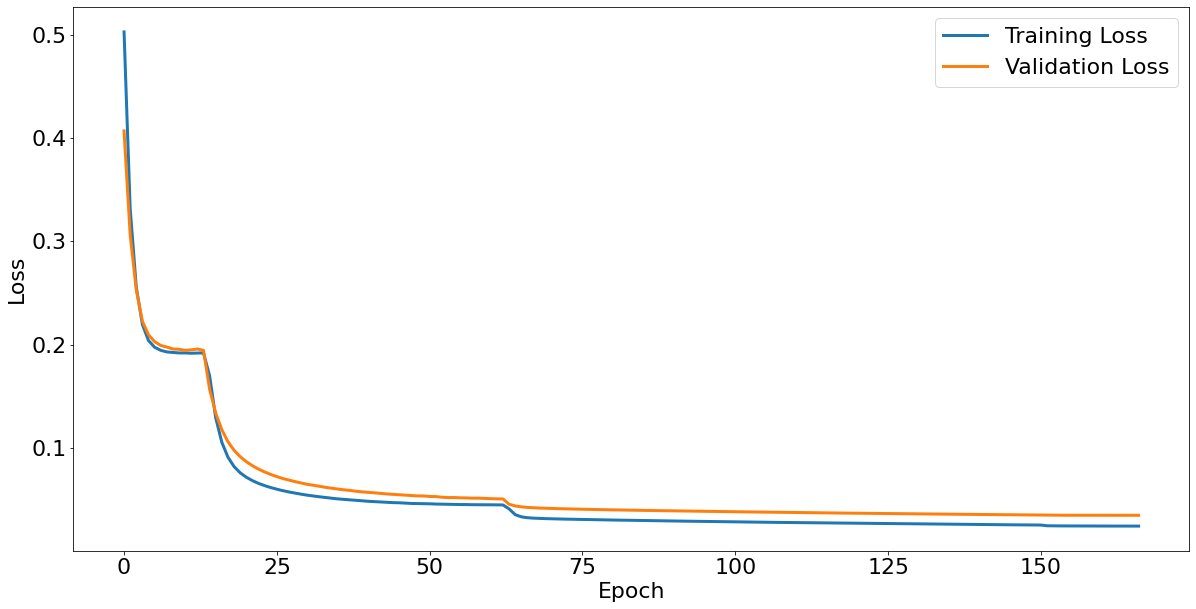
\includegraphics[width=.9\textwidth]{figures/ARAMNet-loss.png}
    \caption{Training and Validation learning curve for ARAMNet}
    \label{Figure:ARAMNet-Learning-Curve} 
\end{figure}